Consider the following IP problem and its standard form

\begin{minipage}[c]{0.4\textwidth}
\begin{align*}
\text{(IP)} \quad z = \text{max} \quad & 4x_1 - x_2      \\
                   \st \quad & 7x_1 -  2x_2    \leq 14\\
                             & x_2 \leq 3 \\
		       		         & 2x_1 -     2x_2 \leq 3 \\
		     	             & x_1,x_2 \in \integers_+
\end{align*}
\end{minipage}
\begin{minipage}{0.5\textwidth}
\begin{table}[H]
	\centering
	\begin{tabular}{V{0.3cm} V{0.6cm} V{0.2cm} r V{0.1cm} V{0.1cm} V{0.4cm} V{0.2cm} r r}
        $\text{(IP)}$  & z =   &     max & \multicolumn{3}{c}{$4x_1 - x_2$}                \vspace{5pt}               \\
		               & $\st$ &  7$x_1$ &  $+$\ 2$x_2$ & $+ \ x_3$ &           &           & $=$ &  14 &             \\
					   &       &         &        $x_2$ &           & $+ \ x_4$ &           & $=$ &   3 &             \\
					   &       &  2$x_1$ &  $-$\ 2$x_2$ &           &           & $+ \ x_5$ & $=$ &   3 & \vspace{5pt}\\ 
	                   & \multicolumn{8}{c}{$x_1, \dots, x_5 \in \integers_+$}   
	\end{tabular}
\end{table}
\end{minipage}\\

Solve the IP problem by LP-based branch and bound, i.e., use LP relaxations to compute dual (upper) bounds. Use Dual Simplex to efficiently solve the subproblem of each node starting from the optimal basis of the previous node. Recall that the LP relaxation of IP is obtained by relaxing the variables $x_1,\dots,x_5\in \integers_+$ to $x_1,\dots,x_5 \geq 0$.

\emph{Hint:} The initial dual bound $\overline{z}$ is obtained by solving the LP relaxation of IP at the root node $S$. Let $[\underline{z},\overline{z}]$ be the lower and upper bounds of each node. The optimal tableau and the initial Branch \& Bound  tree with only the root node $S$ is shown below. 

\vspace{5pt}

\renewcommand{\arraystretch}{1.2}
\setlength{\tabcolsep}{8pt}

\begin{minipage}{0.72\textwidth}
\begin{tabular}{r|c|ccccc}
       & -$z$  & $x_1$ & $x_2$ & $x_3$ & $x_4$ & $x_5$\\
     \hline
       & -59/7 & 0     & 0     & -4/7  & -1/7  & 0\\
     \hline
$x_1=$ & 20/7 & 1     & 0     &  1/7  & 2/7   & 0\\
$x_2=$ &  3   & 0     & 1     &  0    &  1    & 0\\
$x_5=$ & 23/7 & 0     & 0     & -2/7  & 10/7  & 1 
\end{tabular}
\end{minipage}
\begin{minipage}{0.23\textwidth}
\footnotesize
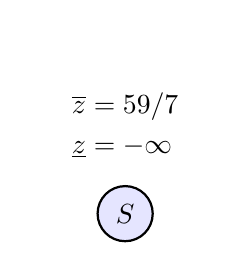
\begin{tikzpicture}[thick, label distance=-1.5mm, level 1/.style={sibling distance=20mm},
					level 2/.style={sibling distance=20mm},  level distance=12mm]

    \tikzstyle{every node}=[draw,circle,minimum size=7mm]

    \node[opacity=1,
    	  fill=blue!10,
    	  label={[label distance=-14pt]above:\begin{tabular}{l} 
    										 $\overline{z}  = 59/7$\\
    										 $\underline{z} = -\infty$
    									     \end{tabular}}](root){$S$};
\end{tikzpicture}
\end{minipage}\\[5pt]

You can proceed by branching on the fractional variable $x_1$ and imposing either $x_1\leq 2$ or $x\geq 3$. This creates two new subproblems $S_1 = S\cap \{x_1\leq 2\}$ and $S_2 = S\cap \{x_1\geq 3\}$ in the branch-and-bound tree that can be solved efficiently using the dual simplex method, starting from the optimal tableau of $S$ shown above, by first adding the new constraint $x_1\leq 2$ for $S_1$ or $x_1\geq 3$ for $S_2$ to the optimal tableau. The dual simplex method can be applied immediately if the new constraint is always written in terms of non-basic variables before adding it to the tableau as a new row, possibly multiplying the constraint by $-1$ if needed. 